\textbf{Problem 3.}

\begin{enumerate}[label=(\roman*),leftmargin=*,itemsep=0mm]
    
    \item The solution to a unit impulse at the origin in an infinite domain has the form
    \begin{align*}
        u(x,t) = \frac{1}{\sqrt{4\pi\kappa t}}\exp(-\frac{x^2}{4\kappa t})
    \end{align*}
    
    We wish to verify that for $t>0$, the above solution is indeed a solution of the heat conduction equation $u_t = \kappa u_{xx}$.
    
    \begin{align*}
        u_t &= -\frac{1}{2t}\frac{1}{\sqrt{4\pi\kappa t}} \exp(-\frac{x^2}{4\kappa t})
        + \frac{x^2}{4kt^2}\frac{1}{\sqrt{4\pi\kappa t}} \exp(-\frac{x^2}{4\kappa t}) \\
        &= \left(-\frac{1}{2t}+\frac{x^2}{4\kappa t}\right) u \\
        u_x &= - \frac{x}{2\kappa t} u \\
        \therefore u_{xx}
        &= - \frac{1}{2\kappa t}u + \left(\frac{x}{2\kappa t}\right)^2 u
        = \left(-\frac{1}{2\kappa t}+\frac{x^2}{4\kappa^2 t}\right) u = \frac{u_t}{\kappa}
    \end{align*}
    
    \item We next perform a change of independent variables $(x,t) \rightarrow (\xi,t')$, where
    \begin{align*}
        \xi = x - Ut, \quad t' = t
    \end{align*}
    
    Therefore, we see that
    \begin{align*}
        u_t &= u_{t'}t'_t + u_{\xi}\xi_t
        = u_{t'} - Uu_{\xi} \\
        u_x &= u_{t'}t'_x + u_{\xi}\xi_x = u_\xi \\
        u_{xx} &= u_{t't'} t_x'^2 + 2u_{t'\xi} \xi_x t'_x + u_{\xi\xi}\xi_x^2 + u_{t'}t'_{xx} + u_{\xi}\xi_{xx} \\
        &= 0 + 0 + u_{\xi\xi} + 0 + 0 = u_{\xi\xi}
    \end{align*}
    
    So the linear convection-diffusion equation is transformed into
    \begin{align*}
        u_t + Uu_x = \kappa u_{xx} \Rightarrow u_{t'} - Uu_{\xi} + Uu_{\xi} = u_{t'} = u_{\xi\xi}
    \end{align*}
    
    The solution of which is
    \begin{align*}
        u(\xi,t') &= \frac{1}{\sqrt{4\pi\kappa t'}}\exp(-\frac{\xi^2}{4\kappa t'}) \\
        \therefore u(x-Ut,t) &= \frac{1}{\sqrt{4\pi\kappa t}}\exp(-\frac{(x-Ut)^2}{4\kappa t})
    \end{align*}
    
    \item We consider discretized forms of the components of the linear convection-diffusion equation as follows:
    \begin{align*}
        u_t &= \frac{\partial u}{\partial t} = \frac{P_i^{n+1} - P_i^n}{\tau} \\
        u_x &= \frac{\partial u}{\partial x} = \frac{P_{i+1}^n - P_{i-1}^n}{2\Delta x} 
        = \frac{P_{i+1}^n - P_{i-1}^n}{2/M} = \frac{M(P_{i+1}^n - P_{i-1}^n)}{2} \\
        u_{xx} &= M^2(P_{i+1}+P_{i_1}-2P_i)
    \end{align*}
    
    Such that we convert the discrete Markov process to:
    \begin{gather*}
        P_i^{n+1} - P_i^n + \left(p-\frac{1}{2}\right)(P_{i+1}^n-P_{i-1}^n)
        = \frac{1}{2}(P_{i+1}+P_{i_1}-2P_i) \\
        \tau u_t + \frac{2p-1}{M} u_x = \frac{2}{M^2}u_{xx} \Rightarrow u_t + \frac{2p-1}{M\tau} = \frac{1}{2M^2\tau}u_{xx}
    \end{gather*}
    
    Comparing against the actual linear convection-diffusion equation, and noting that $t = N\tau$, we have that
    \begin{align*}
        U = \frac{2p-1}{M\tau} = \frac{2p-1}{Mt/N} \Rightarrow Ut &= \frac{(2p-1)N}{M} \\
        \kappa = \frac{1}{2M^2\tau} \rightarrow \kappa t &= \frac{N}{2M^2}
    \end{align*}
    
    Let us now transform $x$ and $t$ to $x_n$ and $t_n$ such that
    \begin{align*}
        x_n = x + c_x, \quad
        t_n = t + c_t
    \end{align*}
    
    Such that when $t=0$)
    \begin{align*}
        u(x_n,0) &= \frac{1}{\sqrt{4\pi\kappa c_t}}
        \exp(-\frac{(x+c_x-Uc_t)^2}{4\kappa c_t}) \\
        &= \frac{1}{\sqrt{2\pi(0.05)^2}}
        \exp(-\frac{(x-0.2)^2}{2(0.05)^2})
    \end{align*}
    
    So, we see that $c_t$ and $c_x$ are:
    \begin{align*}
        c_t &= \frac{2(0.05)^2}{4\kappa} = \frac{1}{800\kappa} \\
        c_x &= -0.2 + Uc_t
    \end{align*}
    
    And therefore, the final equation therefore becomes
    \begin{align*}
        u(x_n,t_n) &= \frac{1}{\sqrt{4\pi\kappa t_n}}
        \exp(-\frac{(x_n-Ut_n)^2}{4\kappa t_n}) \\
        &= \frac{1}{\sqrt{4\pi\kappa (t+c_t)}}
        \exp(-\frac{(x + c_x - U(t + c_t))^2}{4\kappa (t+c_t)}) \\
        &= \frac{1}{\sqrt{4\pi\kappa (t+c_t)}}
        \exp(-\frac{(x - 0.2 - Ut)^2}{4\kappa (t+c_t)})  \\
        &= \frac{1}{\sqrt{4\pi(\kappa t + 1/800)}}
        \exp(-\frac{(x - 0.2 - Ut)^2}{4(\kappa t + 1/800)})
    \end{align*}
    
    So we have the analytical solution for $t=0$ and $t=N\tau$
    \begin{align*}
        u(x,0) &= \frac{20}{\sqrt{2\pi}} e^{-200(x - 0.2)^2} \\
        u(x,N\tau)
        &= \frac{1}{\sqrt{4\pi(N/2M^2 + 1/800)}}
        \exp(-\frac{(x - 0.2 - (2p-1)N/M)^2}{4(N/2M^2 + 1/800)})
    \end{align*}
    
    \begin{figure*}[h!]
    \centering
    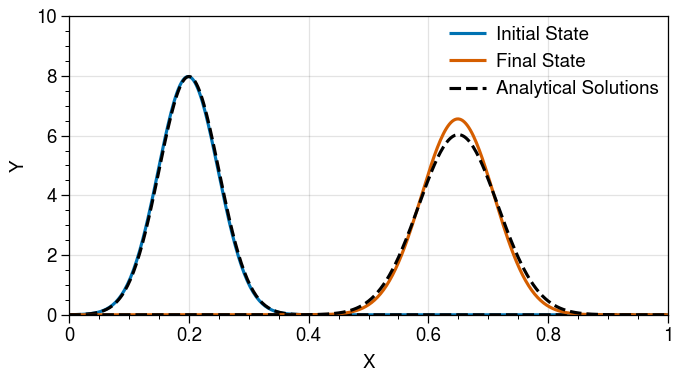
\includegraphics[width=0.8\textwidth]{figures/hw1_qn3.png}\\
    \caption{Plots of our analytic solutions (black-dashed), and initial (blue) and final (red) numerical solutions to the linear convection-diffusion equation.  Here $M=400$, $N=300$ and $p=0.8$.}
    \label{hw1_qn3}
\end{figure*}
    
\end{enumerate}